% CVPR 2024 Paper Template; see https://github.com/cvpr-org/author-kit

\documentclass[10pt,twocolumn,letterpaper]{article}

%%%%%%%%% PAPER TYPE  - PLEASE UPDATE FOR FINAL VERSION
%\usepackage{cvpr}              % To produce the CAMERA-READY version
%\usepackage[review]{cvpr}      % To produce the REVIEW version
 \usepackage[pagenumbers]{cvpr} % To force page numbers, e.g. for an arXiv version

%
% --- inline annotations
%
\usepackage[dvipsnames]{xcolor}
\newcommand{\red}[1]{{\color{red}#1}}
\newcommand{\todo}[1]{{\color{red}#1}}
\newcommand{\TODO}[1]{\textbf{\color{red}[TODO: #1]}}
% --- disable by uncommenting  
% \renewcommand{\TODO}[1]{}
% \renewcommand{\todo}[1]{#1}




\definecolor{cvprblue}{rgb}{0.21,0.49,0.74}
\usepackage[pagebackref,breaklinks,colorlinks,citecolor=cvprblue]{hyperref}

%%%%%%%%% PAPER ID  - PLEASE UPDATE
\def\paperID{*****} % *** Enter the Paper ID here
\def\confName{Xinyu Chen}
\def\confYear{2024}

%%%%%%%%% TITLE - PLEASE UPDATE
\title{Downstream Applications of Open-Vocabulary Visual Perception: \\Scene Understanding}

%%%%%%%%% AUTHORS - PLEASE UPDATE
\author{Xinyu Chen\\
{\tt\small chenxy835@mail2.sysu.edu.cn}
}

\begin{document}
\maketitle
\begin{abstract}

With the rapid development of deep learning and computer vision technologies, visual perception systems have made significant progress in tasks such as image recognition, object detection, and scene understanding. However, traditional visual perception models often rely on predefined closed vocabulary sets, limiting their ability to handle unseen objects and scenes. To overcome this limitation, open-vocabulary visual perception has emerged, enabling the recognition and understanding of a large, potentially unlimited, set of new vocabularies. This significantly enhances the generality and flexibility of visual perception systems. Among the various applications of open-vocabulary visual perception, scene understanding is a key research area. Scene understanding requires not only recognizing individual objects in an image but also understanding the relationships between objects, the semantic structure of the scene, and the context of the overall environment, which is crucial for applications such as autonomous driving, intelligent surveillance, and augmented reality. This paper reviews the downstream applications of open-vocabulary visual perception in scene understanding, focusing on the research presented in three papers: \textit{From Pixels to Graphs: Open-Vocabulary Scene Graph Generation with Vision-Language Models}, \textit{OpenMask3D: Open-Vocabulary 3D Instance Segmentation}, and \textit{OVER-NAV: Elevating Iterative Vision-and-Language Navigation with Open-Vocabulary Detection and Structured Representation}. These papers introduce technologies related to open-vocabulary visual perception in scene understanding, covering various techniques and providing insights into the field.

\end{abstract}    
\section{Introduction}
\label{sec:intro}

\subsection{OVVP}
Open-Vocabulary Visual Perception (OVVP) refers to the ability of computer vision systems to recognize and process new objects and concepts beyond a predefined set of vocabulary. Traditional visual perception systems typically rely on fixed vocabularies for object detection and recognition, exhibiting significant limitations when faced with unseen objects. The goal of OVVP is to enhance the system's adaptability and generality in real-world applications by integrating visual and language models, enabling the system to handle an infinitely expanding set of vocabulary. Key techniques for achieving OVVP include:


\textbf{Vision-Language Models (VLMs)}
VLMs establish semantic connections between visual and textual data through joint training, allowing for the understanding and recognition of new vocabulary. For example, the CLIP (Contrastive Language-Image Pretraining) model maps images and text to a common vector space and uses the similarity between image and text embeddings for object recognition and classification. By leveraging large-scale image-text contrastive learning, VLMs have demonstrated excellent performance in open-vocabulary object recognition tasks.

\textbf{Zero-Shot Learning}
Zero-shot learning is a crucial technique in OVVP, aiming to recognize categories that have not been seen during training. Zero-shot learning utilizes the semantic descriptions of categories (e.g., textual descriptions or attribute information) to map the semantic information of new categories to the visual feature space, enabling the recognition of unseen objects.



\subsection{Scene Understanding}


Scene understanding is a key task in computer vision, aiming to extract meaningful semantic information from images or videos, including object recognition, inference of object relationships, and the semantic structure of the overall scene. Scene understanding involves detecting and classifying individual objects, understanding complex relationships and contexts between objects, and typically requires the completion of the following tasks:

\textbf{Object Detection and Recognition}: Identifying individual objects in images or videos and determining their categories and locations.

\textbf{Scene Classification}: Classifying entire images to identify the scene category they belong to, such as streets, kitchens, forests, etc.

\textbf{Scene Graph Generation (SGG)}: Generating graph structures that describe the objects and their relationships within a scene, where nodes represent objects, and edges represent relationships between objects.

\textbf{Semantic Segmentation}: Classifying each pixel in an image to identify different regions and objects within the image.

\textbf{Instance Segmentation}: Similar to semantic segmentation but further distinguishes between different instances of the same object category within the image.







\subsection{Challenges and Technical Difficulties}

The application of OVVP technology in scene understanding holds great potential but also faces numerous challenges and technical difficulties:

\textbf{Data Annotation and Acquisition}: Training OVVP models requires large-scale, high-quality image-text data. The data annotation process is time-consuming and labor-intensive, often plagued by poor annotation quality and noise. Efficiently acquiring and annotating large-scale multimodal data is a critical challenge.

\textbf{Model Generalization Ability}: Despite the excellent performance of existing VLMs in open-vocabulary object recognition, their generalization ability remains limited when faced with completely unknown or complex scenes and objects.

\textbf{Computational Resources and Efficiency}: Training large-scale VLMs demands significant computational resources and memory, and the efficiency of the inference process also needs optimization. Balancing model performance and computational efficiency is another challenge for the practical application of OVVP technology.


\subsection{Overview of the Articles}

This paper discusses the specific application techniques of OVVP in scene understanding based on three significant articles. The overviews of the three articles are as follows:

\textit{From Pixels to Graphs:Open-Vocabulary Scene Graph Generation with Vision-Language Models \cite{li2024frompixels}}:

This paper proposes a method for generating open-vocabulary scene graphs from pixels using VLMs, transforming images into semantically rich scene graphs. This approach enhances scene understanding by enabling the system to generalize over unseen objects and relationships, producing more accurate and comprehensive scene graphs.

\textit{OpenMask3D: Open-Vocabulary 3D Instance Segmentation \cite{takmaz2023openmask3d}}:

This paper presents a method for open-vocabulary 3D instance segmentation, capable of detecting and segmenting unseen object instances in 3D scenes, significantly improving 3D scene understanding. By combining multimodal data and advanced segmentation algorithms, the system achieves high-precision object recognition and segmentation in complex 3D environments.

\textit{OVER-NAV: Elevating Iterative Vision-and-Language Navigation with Open-Vocabulary Detection and Structured Representation \cite{zhao2024overnav}}:

This paper proposes an iterative vision-and-language navigation method combining open-vocabulary detection and structured representation, enhancing the navigation performance of robots in complex environments. Through open-vocabulary detection technology, robots can recognize and understand unseen environmental features and use structured representation for path planning and decision-making.



\section{Techniques for Scene Understanding}
\label{sec:formatting}




\subsection{Open-Vocabulary Scene Graph Generation}


The paper "From Pixels to Graphs: Open-Vocabulary Scene Graph Generation with Vision-Language Models" introduces a novel framework for open-vocabulary scene graph generation (SGG). The primary goal of SGG is to parse images into graph representations that describe object entities and their relationships within visual scenes. These generated scene graphs serve as structural and interpretable representations for various vision-language tasks, enabling a deeper understanding of the visual content.

Most existing methods have focused on closed-world SGG problems, which cover only a limited subset of the diverse visual relationships found in the real world. This limitation leads to incomplete scene representations and creates domain gaps in downstream vision-language tasks. Traditional SGG methods often suffer from data biases and insufficient labels, resulting in suboptimal performance. While some approaches attempt to address open-vocabulary SGG using vision-language pretraining models, they usually focus on simplified open-vocabulary settings, such as predicate classification for new entities or given entity pairs.


To address these issues, the authors propose an open-vocabulary SGG framework based on image-to-sequence generation, termed PGSG (Pixels to Scene Graph Generation). This framework formulates the SGG task as an image-to-sequence generation problem, leveraging the powerful capabilities of generative vision-language models (VLMs) to generate scene graph sequences. It introduces a fine-tuning strategy based on generative VLMs, offering a more efficient way to utilize the rich visual-language knowledge of pretrained VLMs for relationship-aware representations without additional VLM pretraining.



\begin{figure*}[h]
  \centering
  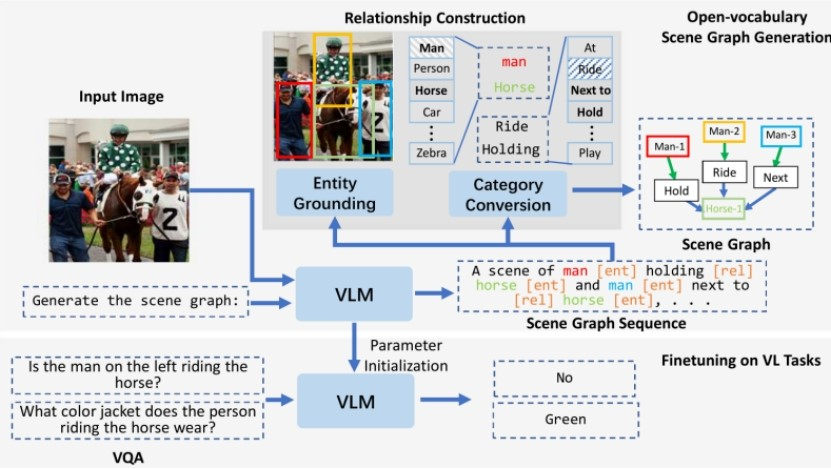
\includegraphics[width=0.7\textwidth]{img/pgsg.jpg}
  \caption{overall pipeline of our PGSG}
\end{figure*}


The PGSG framework comprises three main components:

\textbf{Scene graph prompting}: This component generates sequence representations with relationship-aware tokens, effectively guiding the VLM in capturing relevant visual relationships.

\textbf{Pretrained VLM generating scene graph sequences}: The pretrained VLM generates corresponding scene graph sequences for each input image, translating visual information into structured graph formats.

\textbf{Relationship construction module}: This plug-and-play module uses relationship triplets for entity localization and category conversion. Entity localization predicts entity bounding boxes using an encoder-decoder architecture, while category conversion predicts the transformation from vocabulary space to category space, ultimately generating the output scene graph.


\begin{figure}[h]
    \centering
    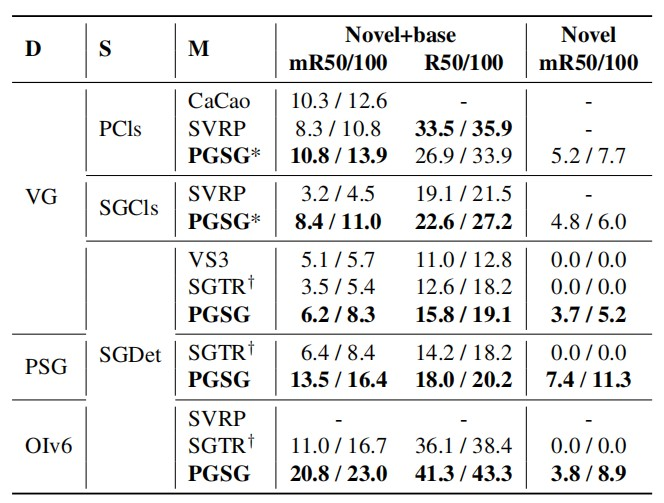
\includegraphics[width=0.5\textwidth]{img/result1_1.jpg} % Adjust the width as needed
    \caption{The open-vocabulary scene graph generation on VG, PSG, and OIV6 datasets}
    \label{fig:pgsg}
\end{figure}


The authors validate their framework on three SGG benchmark datasets \ref{fig:pgsg} (Panoptic Scene Graph, OpenImages-V6, and Visual Genome), achieving state-of-the-art performance. Additionally, they apply the SGG-based VLM to various vision-language tasks such as visual question answering, image captioning, and visual grounding, demonstrating consistent performance improvements. This highlights the effectiveness of their relationship knowledge transfer paradigm in enhancing the interpretability and functionality of vision-language systems.

In summary, this paper proposes a new framework based on generative VLMs to address the general open-vocabulary SGG problem. It introduces scene graph prompting and a plug-and-play relationship-aware transformation module, enabling more efficient model learning and application. The framework demonstrates significant performance improvements in various downstream vision-language tasks, providing new directions and ideas for future research in open-vocabulary visual perception.


\begin{figure*}[h]
  \centering
  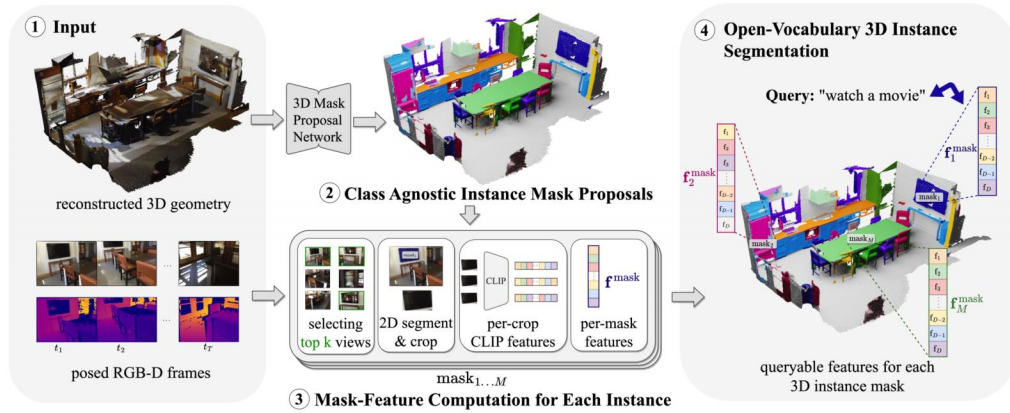
\includegraphics[width=0.7\textwidth]{img/openmark.png}
  \caption{overview of OpenMask3D approach}
\end{figure*}

\subsection{Open-Vocabulary 3D Instance Segmentation}

The paper "OpenMask3D: Open-Vocabulary 3D Instance Segmentation" introduces an innovative technique for open-vocabulary 3D instance segmentation grounded in open-vocabulary visual perception. Traditional 3D instance segmentation methods are constrained to recognizing only predefined object categories that are annotated in the training datasets. This limitation hinders their effectiveness in real-world applications where new and unseen objects frequently appear.

OpenMask3D addresses this limitation through a zero-shot approach, enabling the segmentation of 3D instances based on open-vocabulary descriptions. This method can handle queries that describe previously unseen or novel object attributes, such as geometric shapes, uses, and materials. By doing so, OpenMask3D extends the capabilities of instance segmentation beyond the predefined concepts typically encountered in training data.



OpenMask3D consists of three computational stages:

\textbf{Instance Mask Proposal}: Utilizing a pretrained 3D instance segmentation model’s mask module, OpenMask3D computes category-agnostic instance mask proposals. This step generates initial masks that are not tied to specific object categories, providing a flexible foundation for further processing.

\textbf{Mask Feature Computation}: For each predicted instance mask, OpenMask3D calculates a task-agnostic feature representation using the CLIP model. This process involves selecting the top-k views of the object, obtaining multi-level cropped images, and extracting CLIP features to create a comprehensive feature representation for each mask. This approach ensures that the feature representation captures various aspects of the object from different perspectives.

\textbf{Concept Query Computation}: The final stage involves computing the concept query to obtain the 3D instance segmentation from the previously computed features. This stage leverages the rich, task-agnostic features to match and retrieve object instances based on the similarity to the provided query.


Distinct from existing point-based methods, OpenMask3D emphasizes instance-based feature computation. This focus enhances the system's ability to retrieve object instance masks effectively based on the similarity of features to the query, allowing for more accurate and flexible instance segmentation.

\begin{figure}[h]
    \centering
    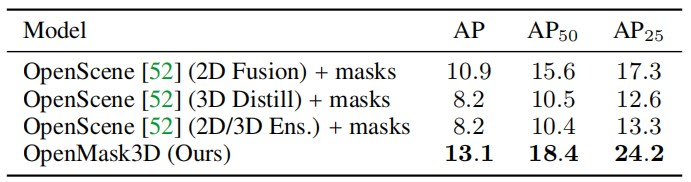
\includegraphics[width=0.5\textwidth]{img/result2_1.jpg}
    \caption{3D instance segmentation results on the Replica dataset}
    \label{fig:Replica}
\end{figure}

\begin{figure*}[h]
    \centering
    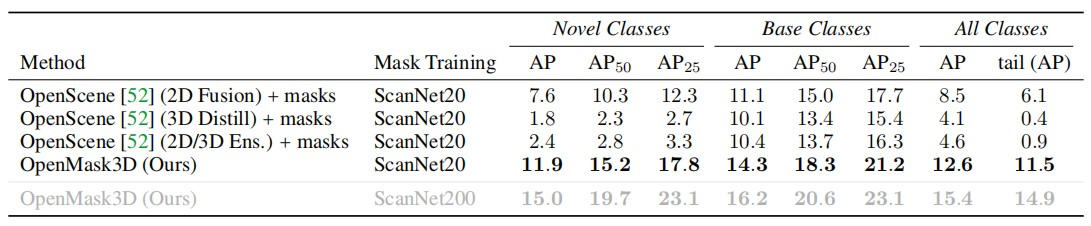
\includegraphics[width=0.9\textwidth]{img/result2_2.jpg}
    \caption{3D instance segmentation results on the ScanNet200 dataset}
    \label{fig:ScanNet}
\end{figure*}

\begin{figure*}[h]
  \centering
  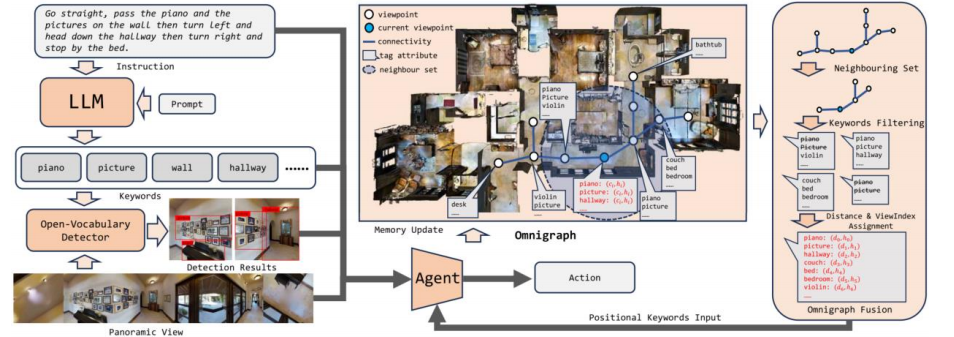
\includegraphics[width=0.8\textwidth]{img/over.png}
  \caption{overview of OVER-NAV method}
\end{figure*}


The authors validate the effectiveness of OpenMask3D on the Replica \ref{fig:Replica} and ScanNet200 \ref{fig:ScanNet} datasets. The results demonstrate that OpenMask3D outperforms existing methods, particularly in handling long-tail distributions of object categories. Qualitative experiments further showcase its capability to segment objects based on diverse attributes and free-form queries, underscoring its versatility and robustness in real-world scenarios.

In summary, similar to the PGSG approach, OpenMask3D leverages vision-language models to transcend the limitations of closed-vocabulary systems. This technique exemplifies the synergistic role of vision-language model methods in advancing open-vocabulary visual perception. Notably, OpenMask3D is the first zero-shot 3D instance segmentation method, significantly broadening the spectrum of recognizable object categories. This advancement enhances the ability of robots to interact with and navigate through unknown environments. It aligns with the objectives of "OVER-NAV," which also improves vision-language navigation through open-vocabulary detection. Together, these methods demonstrate substantial applicability in dynamic and unstructured environments, paving the way for more intelligent and adaptable robotic systems.


\subsection{Vision-and-Language Navigation}

The paper "OVER-NAV: Elevating Iterative Vision-and-Language Navigation with Open-Vocabulary Detection and Structured Representation" introduces a groundbreaking framework for vision-and-language navigation (VLN), termed OVER-NAV. VLN focuses on developing intelligent agents capable of navigating unfamiliar environments by following natural language instructions.

Traditional VLN benchmarks often overlook the agent's memory capabilities, thereby failing to fully leverage cumulative navigation information. While iterative vision-and-language navigation (IVLN) introduces the concept of long-term memory, it still grapples with the challenges of utilizing highly unstructured navigation memory and sparse supervision signals. The OVER-NAV framework effectively addresses these challenges by integrating large language models (LLMs) and open-vocabulary detection (OVD). This integration allows for the extraction and fusion of multimodal information, leading to the construction of a structured memory known as Omnigraph. This significantly enhances the navigation agent’s capability to operate in unseen environments.





The core of the OVER-NAV framework is constructing Omnigraph through OVD. The process includes:

\textbf{Keyword extraction}: LLMs are employed to extract keywords from each navigation instruction. This step ensures that the essential components of the instructions are identified and isolated for further processing.


\textbf{Keyword detection}: As the agent traverses the environment, it continually sends the extracted keywords along with observations made along its path to the OVD. The OVD then detects relevant elements within the environment corresponding to the keywords.

\textbf{Omnigraph construction}: The results from the keyword detection process are stored within the Omnigraph. This structured memory aids the agent in recalling and utilizing parts of the environment’s observations, thus facilitating more informed decision-making.


\textbf{Navigation decision-making}: The real-time computation of scene memory graph information involves feeding the Omnigraph-generated keywords as a text modality into the VLN agent program. This allows the agent to predict navigation actions with greater accuracy in both continuous and discrete environments.


\begin{figure*}[h]
    \centering
    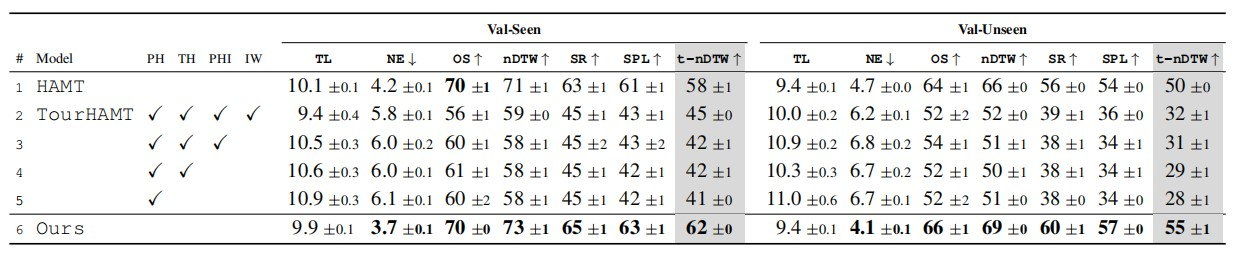
\includegraphics[width=0.8\textwidth]{img/result3_1.jpg} % Adjust the width as needed
    \caption{comparison between OVER-NAV, HAMT and TourHAMT on IR2R}
    \label{fig:IR2R}
\end{figure*}
\begin{figure*}[h]
    \centering
    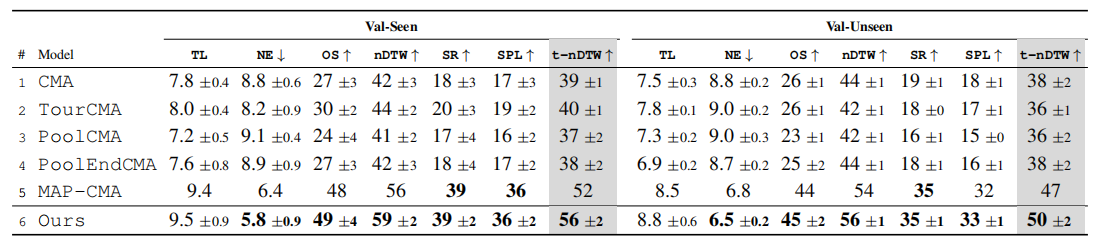
\includegraphics[width=0.8\textwidth]{img/result3_2.jpg} % Adjust the width as needed
    \caption{The performance of OVER-NAV on IR2R-CE}
    \label{fig:IR2R-CE}
\end{figure*}

Experimental results demonstrate the superior performance of OVER-NAV on challenging benchmarks such as IR2R \ref{fig:IR2R} and IR2R-CE \ref{fig:IR2R-CE}. The framework also proves effective in discrete environments, as evidenced by its performance on the REVERIE benchmark. Moreover, the method’s effectiveness is validated when applied to HAMT and MAP-CMA base models, showcasing its versatility and robustness.

In summary, OVER-NAV introduces an innovative framework that incorporates LLMs and OVD into the IVLN paradigm. By introducing a structured representation encoded within Omnigraph, OVER-NAV effectively integrates multimodal information. This leads to significant performance improvements in both discrete and continuous environments, underscoring its potential for advancing the field of vision-and-language navigation.

\section{Applications of Scene Understanding}

Scene understanding is important in several practical applications, and the following are a few key application areas:

    	\textbf{Autonomous Driving}: In the field of autonomous driving, vehicles require real-time and accurate perception and understanding of the surrounding environment to make safe driving decisions. Scene understanding technologies assist autonomous driving systems in identifying objects such as vehicles, pedestrians, and traffic signs on the road, and understanding their relationships, thereby enhancing the safety and reliability of autonomous driving.

    	\textbf{Intelligent Surveillance}: Intelligent surveillance systems monitor specific areas using cameras, requiring real-time detection and recognition of anomalies such as intrusion and fighting behaviors. Scene understanding technologies improve the automation of surveillance systems, reduce manual intervention, and enhance monitoring efficiency and accuracy.

    	\textbf{Augmented Reality (AR)}: In augmented reality (AR) applications, scene understanding technologies are used to identify objects and environments in the real world and overlay virtual information on them. For example, in educational and entertainment applications, AR systems can recognize images in textbooks and display related 3D models or animations, enhancing user experience.

	\textbf{Robot Navigation}: Robots performing tasks in complex environments rely on scene understanding technologies to perceive and comprehend the surrounding environment for path planning and obstacle avoidance. For instance, service robots in home environments need to recognize and locate objects such as furniture and appliances to complete tasks like delivery and cleaning.

\section{Conclusion}
This review explores the downstream applications of open-vocabulary visual perception technologies in scene understanding, analyzing three pivotal papers: "OpenMask3D: Open-Vocabulary 3D Instance Segmentation," "From Pixels to Graphs: Open-Vocabulary Scene Graph Generation with Vision-Language Models," and "OVER-NAV: Elevating Iterative Vision-and-Language Navigation with Open-Vocabulary Detection and Structured Representation." These papers demonstrate the latest advancements in the field and their wide-ranging applications.

\textbf{Open-Vocabulary Scene Graph Generation}

The introduction of a scene graph generation framework from image-to-text in open-vocabulary settings has significantly enhanced both the accuracy of scene graph generation and the performance in downstream vision-language tasks, showcasing the robust capabilities of open-vocabulary systems in complex scene understanding.

\textbf{Open-Vocabulary 3D Instance Segmentation}

OpenMask3D proposes a two-stage method based on the CLIP model for open-vocabulary 3D instance segmentation. It achieves this through category-agnostic mask proposals and multi-view feature aggregation, overcoming the limitations of traditional closed-vocabulary methods and significantly improving system performance in handling novel and diverse objects.

\textbf{Open-Vocabulary Navigation}

OVER-NAV integrates large language models and open-vocabulary detection techniques to propose a new iterative vision-and-language navigation framework. By constructing the structured memory Omnigraph, this approach markedly enhances the navigation capabilities of agents in unknown environments. This method underscores the importance of multimodal information fusion and demonstrates its potential applications in navigation tasks.


In summary, open-vocabulary visual perception technologies exhibit tremendous potential and extensive applications in scene understanding. By leveraging advanced techniques such as vision-language models, open-vocabulary detection, and structured representations, these methods surpass the limitations of traditional closed-vocabulary systems, providing more flexible and intelligent solutions. Future research should continue exploring these technologies across various domains to further advance the development of visual perception and artificial intelligence.


{
    \small
    \bibliographystyle{ieeenat_fullname}
    \bibliography{main}
}

\end{document}
